\chapter{Electrodinámica}

\section{Ley de inducción de Faraday}

Faraday\footnote{Michael Faraday (1791-1867): físico y químico británico. Ver \url{http://es.wikipedia.org/wiki/Michael_Faraday}.} encontró experimentalmente (1831) que \textit{si el flujo magnético a través de una espira cerrada varía en el tiempo, se induce una corriente sobre una espira}. Si el flujo es constante, se observa que la corriente desaparece. La \textbf{ley de Faraday} se escribe como
\begin{equation}\label{faraday}
\varepsilon_{\rm ind}=-K\frac{d\Phi}{dt},
\end{equation}
donde $\varepsilon_{\rm ind}$ es la fuerza electromotriz (f.e.m.) \textit{inducida} en la espira. El signo menos describe la dirección de la corriente inducida, dada por la \textbf{ley de Lenz}. Aquí $K$ es una constante que depende del sistema de unidades usado. En el Sistema Internacional es una cantidad adimensional, que determinaremos más adelante.

En términos de campos, se genera un campo eléctrico $\vec{E}$ que es el que hace mover las cargas en la espira, es decir,
\begin{equation}
\oint_{\cal\partial S}\vec{E}\cdot d\vec{\ell}=\varepsilon_{\rm ind}.
\end{equation}
Con esto, podemos escribir (\ref{faraday}) como
\begin{equation}
\oint_{\cal \partial S}\vec{E}\cdot d\vec{\ell}=-K\frac{d\ }{dt}\int_S\vec{B}\cdot
d\vec{S}.
\end{equation}
En general, la superficie puede variar en el tiempo. Si éste \textit{no} es el caso, y $S$
es constante, entonces podemos deducir que
\begin{equation}\label{ley-faraday0}
\vec\nabla\times\vec{E}=-K\frac{\partial\vec{B}}{\partial t}.
\end{equation}
Considere ahora el caso en que la espira se mueve \textit{rígidamente}, es decir, que la velocidad de los puntos de la espira es independiente de la posición (puede, sin embargo, depender del tiempo).
Entonces el cambio del flujo por la superficie, entre los tiempos $t$ y $t+dt$, puede calcularse como sigue:
\begin{eqnarray}
 d\Phi &=& \Phi(t+dt)-\Phi(t)\\
&=&
\int_{S(t+dt)}B_i(\vec{x}+\vec{v}dt,t+dt)dS_i-\int_{S(t)}B_i(\vec{x},t)dS_i\\
&=&\int_{S(t+dt)}\left[B_i(\vec{x},t)+dt\,v_j\,\partial_jB_i(\vec{x},
t)+dt\,\partial_tB_i(\vec{x},t)\right ] dS_i-\int_{S(t)}B_i(\vec{x},t)dS_i\\
&=&\int_S\left[B_i(\vec{x},t)+dt\,v_j\,\partial_jB_i(\vec{x},
t)+dt\,\partial_tB_i(\vec{x},t)\right ] dS_i-\int_SB_i(\vec{x},t)dS_i\\
&=&dt\int_S\left[v_j\,\partial_jB_i(\vec{x},t)+\partial_tB_i(\vec{x},t)\right
] dS_i.
\end{eqnarray}
En la penúltima igualdad usamos el hecho que el elemento de superficie $dS_i$ sobre la superficie $S(t)$ y $S(t+dt)$ son iguales, ya que la superficie se mueve rígidamente (es decir, con igual velocidad en cada punto). Así obtenemos que
\begin{equation}\label{dPhidt0}
 \frac{d\Phi}{dt}=\int_S\left[v_j\,\partial_jB_i(\vec{x},t)+\partial_tB_i(\vec
{x},t)\right] dS_i.
\end{equation}
Usamos ahora la identidad
\begin{equation}
\varepsilon_{ijk}\partial_j(\varepsilon_{klm}B_lv_m)\equiv
v_j(\partial_jB_i)-v_i(\partial_jB_j),
\end{equation}
y la ley (\ref{divB}) (que suponemos válida incluso en el caso dinámico) para reescribir (\ref{dPhidt0}) como
\begin{eqnarray}
 \frac{d\Phi}{dt}&=&\int_S\left[\partial_tB_i+\varepsilon_{ijk}
\partial_j(\varepsilon_{klm} B_lv_m)\right] dS_i \\
&=& \int_S\partial_tB_i\, dS_i +\oint_{\partial S}\varepsilon_{ijk}
B_jv_k\,dx_i 
\end{eqnarray}
o, en notación vectorial, 
\begin{equation}\label{dFlujodt}
  \frac{d\Phi}{dt}=\int_S\frac{\partial\vec{B}}{\partial
t}\cdot d\vec{S}-\oint_{\partial
S}\left(\vec{v}\times\vec{B}\right)\cdot d\vec{\ell}.
\end{equation}
Apliquemos estos resultados para comparar la descripción, respecto a dos sistemas de referencia inerciales (SRI's), del fenómeno de inducción de corriente en una espira debido a la variación de flujo magnético. Primero, en el SRI $K$ en el que la espira está en reposo y el magneto se mueve tenemos que en cada punto del espacio el campo magnético $\vec{B}$ dependerá del tiempo, por lo que se inducirá un campo eléctrico de acuerdo a (\ref{ley-faraday0}). Este campo eléctrico ejercerá una fuerza $\vec{F}_q=q\vec{E}$ sobre una carga $q$ en la espira, que consideraremos inicialmente en reposo. 

Por otro lado, en un SRI $K'$ con velocidad relativa $\vec{v}$ respecto a $K$ (de modo que en $K'$ el magneto está en reposo) la corriente inducida es debido al movimiento de la espira. Si en este SRI el campo magnético es $\vec{B}'(x)$, no existe campo eléctrico inducido puesto que $\partial\vec{B}'/\partial t=\vec{0}$. En este SRI la corriente inducida se describe íntegramente debido a la fuerza de Lorentz ejercida por el campo magnético sobre las cargas en la espira, que ahora se mueven con velocidad $-\vec{v}$. La fuerza que actúa sobre la carga es ahora $\vec{F}'_q=-q\vec{v}\times\vec{B'}$. Además, la f.e.m. está dada, usando el resultado (\ref{dFlujodt}) aplicado a este caso, así como la ley de Faraday (\ref{ley-faraday0}), por 
\begin{equation}
\varepsilon'_{\rm ind}=-K\oint_{\partial S}\left(\vec{v}\times\vec{B}'\right)\cdot d\vec{\ell}.
\end{equation}

 Ya que $K$ y $K'$ son SRI's, la aceleración, y por tanto la fuerza que actúa sobre la carga (inicialmente en reposo en $K$), son necesariamente iguales. De lo anterior, es decir $\vec{F}_q=\vec{F}'_q$, vemos que esto sólo es posible si el campo inducido es dado por
 \begin{equation}\label{EvBp}
\vec{E}=-\vec{v}\times\vec{B'}.
\end{equation}
Además, la f.e.m. debe ser la misma, ya que la corriente inducida lo es, por lo que
\begin{align}
\varepsilon_{\rm ind} &= \varepsilon'_{\rm ind}, \\
\oint_{\partial S}\vec{E}\cdot d\vec{\ell} &=-K\oint_{\partial S}\left(\vec{v}\times\vec{B}'\right)\cdot d\vec{\ell}.
\end{align}
Usando ahora (\ref{EvBp}) en el lado izquierdo obtenemos
\begin{equation}
-\oint_{\partial S}\left(\vec{v}\times\vec{B'}\right)\cdot d\vec{\ell} =-K\oint_{\partial S}\left(\vec{v}\times\vec{B}'\right)\cdot d\vec{\ell}.
\end{equation}
Esta relación implica que la constante $K$ debe tener, en el Sistema Internacional de Unidades, el valor $K=1$. 

De esta forma, la ley de Faraday adopta la forma
\begin{equation}
\boxed{\oint_{\cal\partial S}\vec{E}\cdot d\vec{\ell}=-\frac{d\ }{dt}\int_S\vec{B}\cdot
d\vec{S}}
\end{equation}
o, en forma diferencial:
\begin{equation}
\boxed{\vec\nabla\times\vec{E}=-\frac{\partial\vec{B}}{\partial t}.}
\label{ley-faraday}
\end{equation}

%\subsection{Autoinducción}
%\begin{equation}
% L:=\frac{d\Phi}{dI}
%\end{equation}
%\begin{equation}
% \varepsilon_{\rm ind}=-L\frac{dI}{dt}
%\end{equation}


\subsection{Energía del campo magnético}

Consideremos ahora una espira por la que circula una corriente $I$ y el campo magnético \textit{que ella misma produce}. Si $I$ no varía en el tiempo, no existe fem inducida ya que el flujo magnético por la espira permanece constante (suponemos una espira fija, en reposo). Calcularemos la energía necesaria para cambiar la corriente $I$ y el correspondiente campo magnético $\vec{B}$ en una pequeña cantidad. Durante el intervalo de tiempo $dt$ en que la corriente cambia en $dI$ y el campo magnético en $d\vec{B}$, se genera un campo eléctrico inducido y su correspondiente fem $\varepsilon$ (que en general se superponen al campo y fem que mantenían la corriente $I$ fluyendo originalmente). Este campo inducido ``intenta reducir'' el cambio de la corriente (ley de Lenz) y el campo realiza trabajo sobre las cargas en movimiento en la espira. 
%Calcularemos la energía transferida a las cargas que se ponen en movimiento para formar la corriente inducida en una espira, debido a la inducción de Faraday. Para esto, consideraremos una espira que forma una curva cerrada $\cal C$ por la que circula una corriente inducida $I$. 

Dividiremos la curva en elementos de longitud $d\vec{\ell}=d\ell \,\hat{t}$, en los que existe una carga $dq=\lambda d\ell$. El vector unitario $\hat{t}$ está definido de modo que $d\vec{\ell}$ tiene la orientación standard respecto al vector normal $\hat{n}$ a la superficie que encierra la espira. El campo eléctrico $\vec{E}$ ejerce trabajo sobre las cargas $dq$. En un intervalo de tiempo $dt$ el trabajo realizado sobre las cargas $dq$ es entonces 
\begin{align}
dq\,\vec{E}\cdot d\vec{\ell} &= (\lambda d\ell) \vec{E}\cdot (\vec{v}\,dt) \\
&= (\lambda d\ell) \vec{E}\cdot (v\,\hat{t})\,dt \\
&= (\lambda v) \vec{E}\cdot (d\ell\,\hat{t})\,dt \\
&= I(\vec{E}\cdot d\vec{\ell})\,dt.
\end{align}
Aquí hemos identificado la corriente $I=\lambda v$ sobre la espira, y tomado en cuenta que $\vec{v}=v\hat{t}$. Por lo tanto, el trabajo total realizado por el campo sobre las cargas de la espira, en el intervalo de tiempo $dt$, es dado por
\begin{align}
dW &= \oint_{\cal C}dq\,\vec{E}\cdot d\vec{\ell} \\
&= I\oint_{\cal C}(\vec{E}\cdot d\vec{\ell})\,dt \\
&= I\varepsilon\,dt \\
&= -I\frac{d\Phi}{dt}\,dt \\
&= -I\,d\Phi.
\end{align}

A partir de este resultado vemos que la energía (proveniente de fuentes externas) necesaria para cambiar el flujo magnético en una cantidad $d\Phi$, en un sistema con una corriente $I$ es dada por
\begin{equation}\label{dWIdP}
 \boxed{dU=I\,d\Phi.}
\end{equation}
En otras palabras, \textit{un cambio en el valor de la intensidad de campo $\vec{B}$ requiere invertir energía}. En cierto sentido, la ley de Faraday establece una cierta ``inercia'' en el campo magnético, ya que un sistema de cargas y campos tiende a ``resistirse'' al cambio del valor del campo (y su flujo). 
Esto implica además que \textit{es necesario asociar una energía a una cierta configuración de campos y corrientes}, puesto que es necesario invertir energía para establecer estas corrientes y sus campos asociados. Para evaluar esta energía, reescribiremos (\ref{dWIdP}) usando (\ref{PAdx}): la energía $\delta U$ necesaria para variar el potencial vectorial $\vec{A}(x)$ de un sistema de corrientes y campo magnético en $\delta\vec{A}(x)$ es dada por
\begin{align}
 \delta U &= I\oint_{\cal C}\delta\vec{A}\cdot d\vec{\ell} \\
 &= \oint_{\cal C}\delta\vec{A}\cdot Id\vec{\ell} \\
 &= \int_V\delta\vec{A}\cdot \vec{J}_{\rm ext}\,dV. \label{WdAJ}
\end{align}
En el último paso hemos usado la relación (\ref{IdxJdV}) para reescribir la energía en términos de una integral de volumen de la densidad de corriente. Note que la corriente inducida es en general corriente ``externa'' o de ``conducción'', por lo que hemos explicitado en el último término la densidad de corrientes externas $\vec{J}_{\rm ext}$. Además, usando la ley de Amp\`ere para la excitación magnética (\ref{rotHj}), podemos escribir
\begin{align}
 \delta U 
&= \int_{V'} \delta A_i\,\varepsilon_{ijk}\left(\partial_jH_k\right)\,dV \\
&= \varepsilon_{ijk}\int_{V'} \left[\partial_j(H_k\delta A_i)-H_k(\partial_j\delta A_i)\right]dV\\
&= \varepsilon_{ijk}\oint_{\partial V'}H_k\delta
A_i\,dS_j-\varepsilon_{ijk}\int_{V'}H_k(\partial_j\delta A_i)\,dV\\
&= 0+\int_{V'} H_k\,\varepsilon_{kji}(\partial_j\delta A_i)\,dV\\
&= \int_{V'} H_k\,\delta B_k\,dV.
\end{align}
Aquí hemos extendido el dominio de integración a un volumen $V'\to R_3$, es decir, a todo el espacio, usado el teorema de Gauss y considerado que la integral de superficie se anula en el infinito. Con esto, obtenemos la siguiente expresión para la \textit{energía requerida para cambiar la inducción magnética de un sistema en $\delta{\vec B}(x)$}:
\begin{equation}
 \boxed{\delta U=\int_{R^3} \vec{H}(x)\cdot \delta\vec{B}(x)\,dV.}\label{dUB}
\end{equation}
Note la similitud entre las expresiones (\ref{WdAJ}) y (\ref{dUB}) con los resultados (\ref{Wdiel1}) y (\ref{dUE}) para la energía almacenada por un campo eléctrico, respectivamente.

*** Agregar comentario energía y área bajo la curva de gráfico $H$ v/s $B$ ***

Similarmente a lo discutido en el caso eléctrico, la \textit{energía total requerida para aumentar el campo magnético de un sistema desde cero hasta un valor final $\vec{B}$} es 
\begin{equation}
 U=\int_0^1\int_{R^3} \lambda \, \vec{H}(x)\cdot \delta\vec{B}_\lambda(x)\,dV,
\end{equation}
donde $\vec{B}_\lambda(x)$ es el valor de la inducción magnética correspondiente al caso en que la excitación magnética tiene un valor $\vec{H}_\lambda(x)$ igual a una fracción $\lambda$ de la excitación magnética final, es decir, $\vec{H}_\lambda (x)=\lambda\vec{H}_\lambda (x)$ .

En el caso de un \textit{medio magnético lineal}, tendremos que $\vec{B}_\lambda (x)=\lambda\, \vec{B}(x)$ y por lo tanto $\delta\vec{B}_\lambda (x)=d\lambda\,
\vec{B}(x)$, y entonces
\begin{equation}\label{UHB}
 \boxed{U=\frac{1}{2}\int_{R^3} \vec{H}(x)\cdot\vec{B}(x)\,dV }
\end{equation}
o, alternativamente, 
\begin{equation}
 \boxed{U=\frac{1}{2}\int_{R^3} \vec{A}\cdot \vec{J}\,dV.}
\end{equation}

Usando (\ref{UHB}) podemos escribir la energía almacenada en un sistema de campo magnético (y corrientes) como la integral de una \textbf{densidad de energía magnética}
\begin{equation}
 \boxed{U=\int_{R^3} u_B(x)\,dV, \qquad u_B(x):=\frac{1}{2}\vec{H}(x)\cdot\vec{B}(x).}
\end{equation}
En el caso particular de medio lineales e isótropos la densidad de energía magnética se reduce a
\begin{equation}
 u_B(x)=\frac{\mu}{2}\vec{H}^2(x)=\frac{1}{2\mu}\vec{B}^2(x).
\end{equation}


\subsection{Fuerzas y torques sobre circuitos magnéticos*}
%\begin{equation}
%\boxed{F_i=-\left(\frac{\partial U}{\partial x_i}\right) ,} \label{FQB}
%\end{equation}
%
%\begin{equation}
% \boxed{\vec{\tau}\cdot\hat{n}=-\left(\frac{\partial U}{\partial\theta}\right).}
%\end{equation}

\section{Ecuaciones de Maxwell}
Hasta el momento,
\begin{align}
\vec\nabla\cdot\vec{D} & =\rho ,\label{cmax1}\\
\vec\nabla\cdot\vec{B}  & =0 ,\label{cmax2}\\
\vec\nabla\times\vec{H}  & =\vec{J} ,\label{cmax3}\\
\vec\nabla\times\vec{E}  & =-\frac{\partial\vec{B}}{\partial t} .\label{cmax4}
\end{align}
Note que aquí hemos suprimido, para no recargar la notación, la designación ``${\rm ext}$'' en la densidad de carga y corriente externa.

Vemos que (\ref{cmax3}) implica $\vec\nabla\cdot\vec{J}=0$, que es una condición que \textit{no es válida en general}, sino que sólo en los casos, de acuerdo a (\ref{eccont}), en que ${\partial\rho}/{\partial t}=0$. Esto lleva a pensar que (al menos) la ecuación (\ref{cmax3}) no es válida en el caso dinámico más general en el que las densidades de carga y corriente, y por lo tanto los campos eléctricos y magnéticos, varían en el tiempo.

Maxwell\footnote{James Clerk Maxwell (1831-1879): Físico escocés. Ver \url{http://es.wikipedia.org/wiki/James_Clerk_Maxwell}.} (1861) generalizó la ecuación (\ref{cmax3}) de modo que sea compatible con (\ref{cmax1}) y la ley de conservación de la carga eléctrica,
es decir, con la ecuación de continuidad (\ref{eccont}). Usando (\ref{cmax1}), que suponemos por tanto válida en el caso general, podemos escribir (\ref{eccont}) como
\begin{eqnarray}
 0&=&\frac{\partial\rho}{\partial t}+\vec{\nabla}\cdot\vec{J}\\
&=& \frac{\partial\ }{\partial
t}\left(\vec\nabla\cdot\vec{D}\right)+\vec{\nabla}\cdot\vec{J}\\
&=& \vec\nabla\cdot\left[\frac{\partial\vec{D}}{\partial t}
+\vec{J}\right].
\end{eqnarray}
De aquí vemos que en el caso de corrientes generales (no-estáticas), $\vec{J}$ tiene divergencia no nula, pero la combinación $\vec{J}+{\partial\vec{D}}/{\partial t}$ \textit{siempre tiene divergencia nula}. A partir de esta observación, Maxwell \textit{postuló} que el lado derecho de la ecuación (\ref{cmax3}) debía ser reemplazada por la combinación $\vec{J}+{\partial\vec{D}}/{\partial t}$. En otras palabras, Maxwell postuló que a la densidad de corriente debería agregarse el término ${\partial\vec{D}}/{\partial t}$, llamado \textit{corriente de desplazamiento}.

Con esto, las ecuaciones de Maxwell adoptan la forma:
\begin{align}
\vec\nabla\cdot\vec{D} & =\rho ,\label{max1}\\
\vec\nabla\cdot\vec{B}  & =0 ,\label{max2}\\
\vec\nabla\times\vec{H}  & =\vec{J}+\frac{\partial\vec{D}}{\partial
t} ,\label{max3}\\
\vec\nabla\times\vec{E}  & =-\frac{\partial\vec{B}}{\partial t}.\label{max4}%
\end{align}

Estas ecuaciones son completadas con las relaciones constitutivas entre
$\vec{E}$ y $\vec{D}$, y entre $\vec{B}$ y $\vec{H}$, así como con la expresión de la (densidad de) fuerza de Lorentz:
\begin{equation}
\vec{f}=\rho\vec{E}+\vec{J}\times\vec{B}.
\end{equation}

\section{Conservación de la energía y vector de Poynting}\label{sec:energia}
Calculamos el producto escalar de $\vec{E}$ con la ecuación (\ref{max3}).
Usando notación tensorial, obtenemos:
\begin{equation}
 E_i\frac{\partial D_i}{\partial t}
-E_i\,\varepsilon_{ijk}\partial_jH_k+E_iJ_i=0.
\end{equation}
Análogamente, el producto escalar entre $\vec{H}$ con la ecuación
(\ref{max4}) implica,
\begin{equation}
H_i\frac{\partial B_i}{\partial t} +H_i\varepsilon_{ijk}\partial_jE_k=0.
\end{equation}
Sumando estas ecuaciones, obtenemos
\begin{align}
0 &= E_i\frac{\partial D_i}{\partial t}+H_i\frac{\partial B_i}{\partial t}
-E_i\varepsilon_{ijk}\partial_jH_k+E_iJ_i+H_i\varepsilon
_{ijk}\partial_jE_k\\
 &= E_i\frac{\partial D_i}{\partial t}+H_i\frac{\partial B_i}{\partial
t}+E_iJ_i+\varepsilon_{ijk}\left(H_i\partial_jE_k-E_i\partial_jH_k\right)\\
 &= E_i\frac{\partial D_i}{\partial t}+H_i\frac{\partial B_i}{\partial
t}+E_iJ_i+\varepsilon_{ijk}\left(H_i\partial_jE_k+E_k\partial_jH_i\right)\\
 &= E_i\frac{\partial D_i}{\partial t}+H_i\frac{\partial B_i}{\partial
t}+E_iJ_i+\partial_j(\varepsilon_{jki}E_kH_i).
\end{align}
En resumen, las ecuaciones de Maxwell (\ref{max3}) y (\ref{max4}) implican que
\begin{equation}
\boxed{\vec{E}\cdot\frac{\partial \vec{D}}{\partial
t}+\vec{H}\cdot\frac{\partial\vec{B}}{\partial t}+
\vec\nabla\cdot(\vec{E}\times\vec{H})
+\vec{E}\cdot\vec{J}=0.} \label{cEem0}
\end{equation}
Es útil definir el \textit{vector de Poynting}\footnote{John Henry Poynting (1852-1914): físico inglés. Ver \url{http://es.wikipedia.org/wiki/John_Henry_Poynting} $\leftarrow$ \textbf{Esta página podría ser mejorada considerablemente, traduciendo la correspondiente en inglés!. ?`voluntari@s?}} como
\begin{equation}\label{defPoy}\marginnote{Vector de Poynting}
\boxed{\vec{S}:=\vec{E}\times\vec{H}.}
\end{equation}
En un pequeño intervalo de tiempo $dt$ los campos cambian (en cada punto fijo del espacio) en las pequeñas cantidades dadas por $d\vec{D}=dt\,({\partial \vec{D}}/{\partial t})$ y
$d\vec{B}=dt\,({\partial \vec{B}}/{\partial t})$. Entonces podemos escribir
\begin{equation}
\vec{E}\cdot
d\vec{D}+\vec{H}\cdot d\vec{B}+\vec\nabla\cdot\vec{S}\,dt+\vec{E}\cdot\vec{J}\,
dt=0,
\end{equation}
que, integrado en un volumen $V$ conduce a 
\begin{equation}
\boxed{\int_V\left[\vec{E}\cdot d\vec{D}+\vec{H}\cdot
d\vec{B}\right]dV+\oint_{\partial V}
\vec{S}\cdot d\vec{S}\,dt+\int_V\vec{E}\cdot\vec{J}\,
dVdt=0.} \label{cEem1}
\end{equation}
Identificamos el último término como el \textbf{trabajo realizado por el campo eléctrico sobre las corrientes}, es decir, la energía transferida del campo a las cargas (o viceversa, dependiendo del signo). Además, de acuerdo a los resultados previos (\ref{dUE}) y (\ref{dUB}) la primera integral puede interpretarse como el \textbf{cambio total de la energía almacenada en forma de campo eléctrico y magnético}, en el volumen $V$. Finalmente, interpretamos la integral de superficie como la \textbf{energía electromagnética neta que fluye a través de la superficie $\partial V$}. En otras palabras, interpretamos el vector de Poynting como la \textit{densidad de flujo de energía} electromagnética (la energía electromagnética transportada por unidad de superficie y unidad de tiempo). De esta forma, (\ref{cEem1}) es una \textit{ecuación de balance (o conservación) de la energía}.

En el caso particular de \textit{medios lineales, no disipativos, y con susceptibilidades
independientes del tiempo}, es decir, tales que
\begin{equation}
D_i=\varepsilon_{ij}E_j, \qquad \partial_t\varepsilon_{ij}=0, \qquad \varepsilon_{ij}=\varepsilon_{ji},
\end{equation}
\begin{equation}
B_i=\mu_{ij}H_j, \qquad \partial_t\mu_{ij}=0, \qquad \mu_{ij}=\mu_{ji},
\end{equation}
podemos reescribir:
\begin{equation}
 \vec{E}\cdot\frac{\partial \vec{D}}{\partial
t}=\frac{1}{2}\frac{\partial\ }{\partial t}\left(\vec{E}\cdot\vec{D}\right),
\qquad
 \vec{H}\cdot\frac{\partial \vec{B}}{\partial
t}=\frac{1}{2}\frac{\partial\ }{\partial t}\left(\vec{H}\cdot\vec{B}\right).
\end{equation}
Con esto, (\ref{cEem0}) es equivalente a
\begin{equation}
\boxed{\frac{\partial u}{\partial
t}+\vec\nabla\cdot\vec{S}+\vec{E}\cdot\vec{J}=0 ,} \label{econtEem}
\end{equation}
donde hemos definido la \textit{densidad de energía del campo
electromagnético}:
\begin{equation}\label{uDEHB}
\boxed{u:=\frac{1}{2}\left(\vec{D}\cdot\vec{E}+\vec{H}\cdot\vec{B}\right).}
\end{equation}
La versión integral de (\ref{econtEem}) es
\begin{equation}\label{balanceEem}
\boxed{\frac{d\ }{dt}\left(E^{\rm em}_V+E^{\rm mec}_V\right)+\oint_{\partial
V}\vec{S}\cdot d\vec{S}=0 ,}
\end{equation}
donde
\begin{equation}
E^{\rm em}_V=\int_V u\,dV
\end{equation}
es la \textbf{energía electromagnética} y, de acuerdo al \textit{teorema de trabajo-energía} \textit{en el caso que no existan otras fuerzas que realicen trabajo sobre las cargas},
\begin{equation}
 \frac{d\ }{dt}E^{\rm mec}_V=\int_V\vec{E}\cdot\vec{J}\,dV
\end{equation}
es la variación de energía mecánica total de las cargas contenidas en $V$.

De esta forma podemos interpretar \eqref{balanceEem} como una expresión de balance de energía. La energía total $E^{\rm em}_V+E^{\rm mec}_V$ en un volumen dado $V$, compuesta de la suma de la energía del campo electromagnético y de la energía mecánica de las cargas en $V$, es constante sólo si el flujo neto de energía transportada por el campo electromagnético en la superficie $\partial V$ es nula. Por otro lado si, por ejemplo, el campo electromagnético generado por las cargas en $V$ logra producir un flujo neto $\oint_{\partial V}\vec{S}\cdot d\vec{S}$ positivo a través de $\partial V$, entonces la energía total en $V$ necesariamente disminuirá.

\section{Conservación del momentum lineal}\label{sec:momentum}
La \textbf{fuerza total que el campo electromagnético ejerce sobre las cargas} contenidas en un volumen $V$ es dada por la fuerza de Lorentz:
\begin{equation}
\vec{F}_{\rm em}=\int_V\left(\rho\vec{E}+\vec{J}\times\vec{B}\right)dV .
\end{equation}
Consideremos el integrando de la expresión anterior (es decir, la densidad de fuerza) y reemplacemos las fuentes $\rho$ y $\vec{J}$ usando las ecuaciones de Maxwell inhomogéneas (\ref{max1}) y (\ref{max3}). Con esto, tenemos que
\begin{eqnarray}
f_i&=&\rho E_i+\varepsilon_{ijk}J_jB_k \\
&=&(\partial_jD_j)E_i+\varepsilon_{ijk}(\varepsilon_{
jlm}\partial_lH_m-\partial_tD_j)B_k  \\
&=& \partial_j(D_jE_i)-D_j\partial_jE_i +
(\partial_kH_i)B_k-(\partial_iH_k)B_k-\varepsilon_{ijk}(\partial_tD_j)B_k \\
&=& \partial_j(D_jE_i)-D_j\partial_jE_i +
\partial_k(H_iB_k)-H_i(\partial_kB_k) \nonumber\\
&& -\partial_i(H_kB_k)+H_k(\partial_iB_k)
-\partial_t(\varepsilon_{ijk} D_jB_k)
+\varepsilon_{ijk} D_j(\partial_tB_k) \\
%&=&\partial_j(E_iD_j+H_iB_j-\delta_{ij}H_kB_k)
%-D_j\partial_jE_i+H_j(\partial_iB_j) \nonumber\\
%&& -\partial_t(\varepsilon_{ijk} D_jB_k)
%+\varepsilon_{ijk} D_j(\partial_tB_k) \\
&=&\partial_j(E_iD_j+H_iB_j-\delta_{ij}H_kB_k)
-D_j\partial_jE_i+H_j(\partial_iB_j) \nonumber\\
&& -\partial_t(\varepsilon_{ijk}
D_jB_k)-\varepsilon_{ijk} D_j(\varepsilon_{klm}\partial_lE_m) \\
&=&\partial_j(E_iD_j+H_iB_j-\delta_{ij}H_kB_k)
-D_j\partial_jE_i+H_j(\partial_iB_j) \nonumber\\
&& -\partial_t(\varepsilon_{ijk} D_jB_k)-D_j(\partial_iE_j) +D_j(\partial_jE_i)\\
&=&\partial_j(E_iD_j+H_iB_j-\delta_{ij}H_kB_k)-\partial_t(\varepsilon_{ijk}
D_jB_k)+H_j(\partial_iB_j)- D_j(\partial_iE_j). \label{flc}
\end{eqnarray}
En el caso de medios \textit{lineales, homogéneos y no disipativos}, es decir, para medios tales que
\begin{equation}
 D_i=\varepsilon_{ij}E_j, \qquad \partial_k\varepsilon_{ij}=0, \qquad \varepsilon_{ij}=\varepsilon_{ji},
\end{equation}
\begin{equation}
 B_i=\mu_{ij}H_j, \qquad \partial_k\mu_{ij}=0,\qquad \mu_{ij}=\mu_{ji},
\end{equation}
podemos escribir
\begin{equation}
 \partial_i(D_jE_j)=\varepsilon_{jk}\partial_i(E_kE_j)=2\varepsilon_{jk}
E_k(\partial_i E_j)=2D_j(\partial_i E_j),
\end{equation}
es decir,
\begin{equation}
 D_j(\partial_i E_j)=\frac{1}{2}\partial_i(D_jE_j). \label{idl1}
\end{equation}
Análogamente,
\begin{equation}
 H_j(\partial_i B_j)=\frac{1}{2}\partial_i(H_jB_j). \label{idl2}
\end{equation}
Reemplazando (\ref{idl1}) y (\ref{idl2}) en los últimos dos términos de
(\ref{flc}), encontramos
\begin{equation}
 \rho E_i+\varepsilon_{ijk}J_jB_k
=\partial_j\left[E_iD_j+H_iB_j-\frac{1}{2}\delta_{ij}\left(
E_kD_k+H_kB_k\right)\right]-\partial_t(\varepsilon_{ijk}D_jB_k).
\end{equation}
Definimos la \textbf{densidad de momentum} del campo, $\pi_i$, y (dependiendo de las convenciones, el negativo de) el \textbf{tensor de tensiones de Maxwell}, $T_{ij}$, por
\begin{equation}
\boxed{\pi_i:=\varepsilon_{ijk}D_jB_k,}
\end{equation}
\begin{equation}
 \boxed{T_{ij}:=\frac{1}{2}\delta_{ij}\left(E_kD_k+B_kH_k\right)-E_iD_j-H_iB_j,}
\end{equation}
y entonces
\begin{equation}
\boxed{f_i+\frac{\partial\pi_i }{\partial t}+\partial_jT_{ij}=0.} \label{lcm}
\end{equation}
Integrando (\ref{lcm}) en un volumen $V$ y usando el teorema de Gauss,
encontramos
\begin{equation}
\boxed{F^{\rm em}_i+\frac{d\ }{dt}P_i^{\rm em}+\oint_{\partial
V}T_{ij}\,dS_j =0,} 
\end{equation}
donde $F^{\rm em}_i$ es la fuerza electromagnética total actuando sobre las cargas en $V$, y
\begin{equation}\marginnote{mom. lineal del campo}
 \boxed{P_i^{\rm em}:=\int_V \pi_i\,dV.} \label{defpem}
\end{equation}

Si $\vec{F}_{\rm em}$ coincide con la \textit{fuerza total} sobre las cargas (por ejemplo, si las únicas fuerzas involucradas son electromagnéticas, o si la fuerza neta de origen no electromagnético se anula) entonces, usando la \textit{segunda ley de Newton}, tenemos que $\vec{F}_{\rm em}=d\vec{P}_{\rm mec}/dt$, donde $\vec{P}_{\rm mec}$ es el \textbf{momentum lineal total de las cargas} en $V$ (mecánico). Bajo estas condiciones, podemos escribir
\begin{equation}
\boxed{\frac{d\ }{dt}\left(P_i^{\rm mec}+P_i^{\rm em}\right)+\oint_{\partial
V}T_{ij}\,dS_j =0.} \label{licml}
\end{equation}
En casos en que los campos se anulan en $\partial V$, la relación
(\ref{licml}) expresa que $P_i^{\rm mec}+P_i^{\rm em}$ es conservado. Esto
permite interpretar (\ref{defpem}) como el \textbf{momentum lineal total del
campo electromagnético en el volumen} $V$. En el caso general podemos entonces interpretar la integral $\oint_{\partial V}T_{ij}\,dS_j $ como el \textbf{flujo neto de momentum por unidad de tiempo
a través de} $\partial S$. Consecuentemente, el tensor de Maxwell $T_{ij}$
será interpretado como el tensor \textbf{densidad de flujo de momentum lineal}, y en particular representa el momentum en la dirección $i$ que se transfiere en la dirección $j$, por unidad de tiempo y área. Equivalentemente, $-T_{ij}n_j$ ($dS_j=n_jdS$)
representa la \textit{fuerza por unidad de área} (tensión) que actúa sobre el sistema
de cargas y campos en $V$.

La expresión (\ref{licml}) puede ser usada para calcular la fuerza que actúa
sobre cargas en presencia de campos electromagnéticos. Por ejemplo,

\begin{center}
*** EJEMPLO CONDENSADOR PLACAS PARALELAS ***
\end{center}

\textbf{Para un medio lineal \textit{e isótropo}, el tensor de Maxwell es simétrico
$T_{ij}=T_{ji}$} y la densidad de momentum es proporcional al vector de
Poynting, $\vec{\pi}=\varepsilon\mu\,\vec{S}$, de modo que la dirección del
momentum de campo coincide con la del flujo de energía de
éste.

\section{Conservación del momentum angular*}\label{sec:momentum_angular}
Análogamante al caso del momentum lineal, buscamos una ecuación de balance/conservación del momento angular. El término análogo a la (densidad de) fuerza de Lorentz $f_i$ y que determina (si no hay otras fuerzas involucradas) el cambio del momentum lineal de las cargas, es ahora la \textbf{densidad de torque} (torque que el campo realiza sobre las cargas, por unidad de volumen), y está relacionado (si no hay torques no-electromagnéticos actuando) con el cambio del momento angular de las cargas. 

Recordamos que el momento angular (con respecto al origen del sistema de coordenadas) de una partícula de momentum $\vec{p}$ ubicada en la posición $\vec{x}$ es
\begin{equation}
\vec{L}=\vec{x}\times \vec{p}.
\end{equation}
Su derivada está determinada por el torque actuando sobre la partícula, ya que
\begin{equation}
\frac{d\vec{L}}{dt}=\vec{x}\times \frac{d\vec{p}}{dt}=\vec{x}\times \vec{F},
\end{equation}
donde $\vec{F}$ es la fuerza neta sobre la partícula. Para un sistema con una distribución continua de materia, el momento angular neto de la materia en un volumen $V$ es dado por 
\begin{equation}
\vec{L}_{\rm mec}=\int_V\vec{x}\times d\vec{p},
\end{equation}
y, para materia no-relativista (con velocidades mucho menores que la de la luz), $d\vec{p}=\rho_{\rm m}\vec{v}\,dV$, donde $\rho_{\rm m}(\vec{x},t)$ es la densidad (volumétrica) de masa y $\vec{v}(\vec{x},t)$ es el campo de velocidades. En cualquier caso, podemos escribir $d\vec{p}=\vec{\pi}_{\rm mec}\,dV$ donde $\vec{\pi}_{\rm mec}(\vec{x},t)$ es la densidad (volumétrica) de momentum lineal de la materia. Su derivada temporal es entonces dada por
\begin{equation}
\frac{d\vec{L}_{\rm mec}}{dt} = \int_V\vec{x}\times \frac{\partial\vec{\pi}_{\rm mec}}{\partial t}dV = \int_V\vec{x}\times \vec{f}\,dV, = \int_V\vec{\tau}\,dV,
\end{equation}
donde $ \vec{f}=\partial\vec{\pi}_{\rm mec}/{\partial t}$ es la densidad (volumétrica) de fuerza. La cantidad $\vec{\tau} := \vec{x}\times \vec{f}$ es la densidad de torque (e.d., torque por unidad de volumen respecto al origen del sistema coordenado).

Usaremos la ley de balance de momentum lineal \eqref{lcm} para escribir la densidad de torque en función de las densidades de momentum lineal y su flujo:
\begin{align}
\tau_i &= \epsilon _{ijk}x_{j}f_{k} \\
&=-\epsilon _{ijk}x_{j}\left( \partial _{m}T_{km}+\frac{\partial \pi _{k}}{%
\partial t}\right)  \\
&=-\epsilon _{ijk}x_{j}\left( \partial _{m}T_{km}\right) -\epsilon
_{ijk}x_{j}\left( \partial _{t}\pi _{k}\right) 
\end{align}%
Completando derivadas, podemos escribir:
\begin{equation}
x_{j}\left( \partial _{m}T_{km}\right)  =\partial _{m}\left(
x_{j}T_{km}\right) -(\partial _{m}x_{j})T_{km} = \partial _{m}\left(
x_{j}T_{km}\right) -T_{kj}
\end{equation}
\begin{equation}
x_{j}\left( \partial _{t}\pi _{k}\right)  =\partial _{t}\left( x_{j}\pi
_{k}\right) -(\partial _{t}x_{j})\pi _{k} = \partial _{t}\left( x_{j}\pi
_{k}\right).
\end{equation}
Luego,%
\begin{align}
\tau_i &= -\epsilon _{ijk}\partial _{m}\left(
x_{j}T_{km}\right) +\epsilon _{ijk}T_{kj}-\epsilon
_{ijk}\partial _{t}\left( x_{j}\pi _{k}\right)   \notag \\
&= -\partial _{m}\left( \epsilon _{ijk}x_{j}T_{km}\right) +\epsilon
_{ijk}T_{kj}-\partial _{t}\left( \epsilon _{ijk}x_{j}\pi _{k}\right) 
\end{align}
En el caso de un medio linear \textit{e isótropo} el tensor de tensiones $T_{ij}$ es simétrico, y por lo tanto el término $\epsilon_{ijk}T_{kj}$ se anula. Entonces,
\begin{equation}
\tau_i =-\partial _{m}\left( \epsilon
_{ijk}x_{j}T_{km}\right) -\partial _{t}\left( \epsilon _{ijk}x_{j}\pi
_{k}\right) ,
\end{equation}%
es decir,
\begin{equation}
\partial _{t}\left( \epsilon _{ijk}x_{j}\pi_{k}\right) + \partial _{m}\left( \epsilon_{ijk}x_{j}T_{km}\right)+ \tau_i =0,
\end{equation}%
que interpretamos como la ecuación de balance local de momento angular, similar a \eqref{lcm}. Interpretamos entonces a 
\begin{equation}
l_{i}^{\rm em}:=\epsilon _{ijk}x_{j}\pi_{k}
\end{equation}
o, en notación vectorial,
\begin{equation}
\vec{l}_{\rm em}:=\vec{x}\times\vec{\pi} =\vec{x}\times(\vec{D}\times\vec{B})
\end{equation}
como la \textbf{densidad (volumétrica) de momento angular del campo}, y a
\begin{equation}
\Xi_{im}^{\rm em}:=\epsilon _{ijk}x_{j}T_{km}
\end{equation}
como \textbf{la densidad de flujo del momentum angular}, de modo que
\begin{equation}
\partial _{t}l_{i}^{\rm em} + \partial _{j}\Xi_{ij}^{\rm em} + \tau_i =0.
\end{equation}
La versión integral del balance de momento angular en el sistema, suponiendo ausencia de torques no-electromagnéticos es entonces dada por
\begin{equation}
\frac{d}{dt}\left(L_i^{\rm mec,V}+L_i^{\rm em,V}\right) + \oint_{\partial V}\Xi_{ij}^{\rm em}\,dS_j = 0,
\end{equation}
donde 
\begin{equation}
L_i^{\rm em,V} := \int_V l_{i}^{\rm em}\,dV= \int_V \epsilon _{ijk}x_{j}\pi_{k}\,dV
\end{equation}
es el momento angular total del campo en el volumen $V$.

% Ejemplo 8.4 de Griffiths. Ver pag. 358-361

\section{Ondas Electromagnéticas}

\subsection{Campos electromagnéticos y ecuación de la onda}

Consideremos un \textit{medio lineal, isótropo y homogéneo}. En este caso, a ley de Amp\`ere-Maxwell se reduce a
\begin{equation}
\varepsilon_{ijk}\partial_jB_k=\mu\vec{J}+\varepsilon\mu\frac{\partial E_i}{\partial t}.
\end{equation}
Derivando con respecto al tiempo y usando la ley de Faraday, podemos escribir
\begin{eqnarray}
\mu \frac{\partial J_i}{\partial t}+\varepsilon\mu\frac{\partial^2E_i}{\partial t^2}
&=&\varepsilon_{ijk}\partial_j\frac {\partial B_k}{\partial t} \\
&=&-\varepsilon_{ijk}\partial_j\left(\varepsilon_{klm}\partial_lE_m \right)\\
&=&-\left( \delta_{il}\delta_{jm}-\delta_{im}\delta_{jl}\right)
\partial_j\partial_lE_m\\
&=&\partial_j\partial_jE_i-\partial_j\partial_iE_j.
\end{eqnarray}
Usando la ley de Gauss, $\partial_jE_j=\rho/\varepsilon$, en el segundo término del lado derecho, obtenemos
\begin{equation}\label{EcOihE}
\boxed{\nabla^2\vec{E}-\varepsilon\mu\frac{\partial^2\vec{E}}{\partial t^2}=\frac{1}{\varepsilon}\vec\nabla\rho+\mu\frac{\partial\vec{J}}{\partial t}.}
\end{equation}

Similarmente, calculando la derivada con respecto al tiempo de la ley de Faraday y usando la ley de Amp\`ere-Maxwell, así como el hecho que el campo magnético siempre tiene divergencia nula, es decir \eqref{max2}, encontramos que
\begin{equation}\label{EcOihB}
\boxed{\nabla^2\vec{B}-\varepsilon\mu\frac{\partial^2\vec{B}}{\partial t^2}=-\mu\vec\nabla\times\vec{J}.}
\end{equation}

De esta forma encontramos que \textit{las ecuaciones de Maxwell implican que los
campos eléctrico y magnético satisfacen la ecuación de onda inhomogénea}. Es importante notar que \textit{no todas} las soluciones de la ecuación de onda son necesariamente soluciones de las ecuaciones de Maxwell. En otras palabras, \eqref{EcOihE} y \eqref{EcOihB} son \textit{condiciones necesarias, pero no suficientes} para que los campos satisfagan las ecuaciones de Maxwell.

\textit{En regiones en libres de cargas y corrientes} \eqref{EcOihE} y \eqref{EcOihB} se reducen a la ecuación de onda homogénea para cada componente (cartesiana) de los campos eléctrico y magnético:
\begin{equation}\label{econdaE}
\boxed{\nabla^2E_i-\varepsilon\mu\frac{\partial^2E_i}{\partial t^2}=0.}
\end{equation}
\begin{equation}
\boxed{\nabla^2B_i-\varepsilon\mu\frac{\partial^2B_i}{\partial t^2}=0.}
\label{econdaB}
\end{equation}



\subsection{Ondas electromagnéticas planas monocromáticas}
Consideremos una solución de \textbf{onda plana monocromática polarizada linealmente}:
\begin{equation}
\vec{E}(\vec{x},t)=\vec{E}_0 \cos\left(\vec{k}\cdot\vec{x}-\omega t+\varphi_0\right),
\label{ecuc-max-solu1}%
\end{equation}
donde $\vec{E}_0$, $\vec{k}$, $\omega$ y $\varphi_0$ son constantes. También podemos usar la forma compleja
\begin{equation}
\vec{E}(\vec{x},t)=\operatorname{Re}\left[\vec{E}_{\rm c} e^{i(\vec{k}\cdot\vec{x}-\omega t)}\right],
\label{opmc}%
\end{equation}
donde la amplitud compleja $\vec{E}_{\rm c}$ es dada, en términos de la amplitud real $\vec{E}_0$ y la fase $\varphi_0$, por
\begin{equation}
\vec{E}_{\rm c} = \vec{E}_0 e^{i\varphi_0}.
\end{equation}
Reemplazando (\ref{ecuc-max-solu1}) en (\ref{econdaE}) encontramos que%
\begin{equation}
\left(k^2-\varepsilon\mu\,\omega^2\right)  \vec{E}=0, \qquad k:=|\vec{k}|,
\end{equation}
por lo que las soluciones no triviales requieren que se satisfaga la
\textit{relación de dispersión}:
\begin{equation}
\omega^2=\frac{1}{\varepsilon\mu}\,k^2, \label{rdoem}
\end{equation}
de donde obtenemos la \textbf{velocidad de fase},
$v_{\rm f}:=\omega/k$,
\begin{equation}
v_{\rm f}=\frac{1}{\sqrt{\varepsilon\mu}},
\end{equation}
que además, coincide con la \textbf{velocidad de grupo}, 
\begin{equation}
v_{\rm g} := \frac{\partial\omega}{\partial k}=\frac{1}{\sqrt{\varepsilon\mu}}=v_{\rm g}=:c.
\end{equation}
Esto implica que las ondas electromagnéticas se propagan de forma \textit{no-dispersiva} (en medios lineales, isótropos y homogéneos). 

La \textbf{velocidad de la luz en el medio} ($c$) puede ser escrita en términos de la \textbf{velocidad de la luz en el vacío} ($c_0=1/\sqrt{\varepsilon_0\mu_0}$), la susceptibilidad eléctrica relativa ($\kappa$) y la permeabilidad magnética relativa ($\kappa_{\rm m}$), es decir, usando $\varepsilon=\kappa\varepsilon_0$ y $\mu=\kappa_{\rm m}\mu_0$:
\begin{equation}
c=\frac{c_0}{\sqrt{\kappa\kappa_{\rm m}}}=\frac{c_0}{n}.
\end{equation}
Aquí $n:=\sqrt{\kappa\kappa_{\rm m}}$ es el \textbf{índice de refracción del medio}.

Además, usando (\ref{max4}) obtenemos
\begin{equation}\label{BkE}
 \vec{B}=\frac{1}{\omega}\,\vec{k}\times\vec{E}.
\end{equation}
Similarmente, usando (\ref{max3}) encontramos que
\begin{equation}
 \vec{E}=-\frac{1}{\varepsilon\mu}\frac{1}{\omega}\,\vec{k}\times\vec{B}.
\end{equation}

Estas relaciones implican que $\vec{k}$, $\vec{E}$ y $\vec{B}$ son ortogonales
entre sí y forman (en ese orden) un \textbf{sistema derecho}. Como consecuencia, \textit{una onda electromagnética plana es transversal}, ya que las oscilaciones (de los campos eléctrico y magnético) se producen en el plano ortogonal a la dirección de propagación. Además, los módulos de los campos satisfacen
\begin{equation}
 | \vec{E}|=c\,| \vec{B}| .
\end{equation}
\begin{figure}[!h]
\centerline{\includegraphics[height=3cm]{fig/fig-onda-electromagnetica.pdf}}
\caption{Campos eléctrico y magnético de una onda electromagnética plana monocromática. Adaptada a partir de \href{http://commons.wikimedia.org/wiki/File:Onde_electromagnetique.svg}{esta} figura original.}
\label{ondaem}
\end{figure}

\subsubsection{Vector de Poynting}
Evaluamos el vector de Poynting (\ref{defPoy}) para la solución de onda plana monocromática recién analizada. Usando (\ref{defPoy}), \eqref{BkE} y \eqref{rdoem} podemos escribir
\begin{eqnarray}
 \vec{S}&=&\vec{E}\times\vec{H} \\
&=&\frac{1}{\mu}\,\vec{E}\times\vec{B} \\
&=&\frac{1}{\mu}\,\vec{E}\times\left[\frac{1}{\omega}\,\vec{k}\times\vec{E}
\right] \\
&=&\frac{1}{\mu\omega}\,\vec{E}^2\,\vec{k}\\
&=&\frac{1}{\mu c}\,\vec{E}^2\,\hat{k}. \label{Sop}
\end{eqnarray}
Encontramos de este modo que el campo electromagnético correspondiente a la onda plana estudiada \textit{transporta energía en la dirección del vector de onda $\vec{k}$}. Su magnitud, aunque siempre no-negativa, varía en el tiempo y con la posición, ya que $\vec{E}=\vec{E}(\vec{x},t)$. Como la onda considerada es periódica, de periodo $T=2\pi/\omega$, es usual considerar el \textbf{promedio del vector de Poynting en un periodo de oscilación}\footnote{Si $f(t)$ es una función del tiempo, entonces definimos su promedio entre $t=0$ y $t=T$ como 
\begin{equation}
\left<f\right>:=\frac{1}{T}\int_0^Tf(t)\,dt.
\end{equation}}
Para la onda sinusoidal (\ref{ecuc-max-solu1}) encontramos entonces que
\begin{equation}\label{Sprom}
\langle\vec{S}\rangle=\frac{1}{2\mu c}\,\vec{E}_0^2\,\hat{k}.
\end{equation}
Esto implica que a través de una superficie de área $A$ transversal al vector de onda $\vec{k}$, la onda transporta energía a una tasa (potencia) promedio (en una oscilación) de 
\begin{equation}
 \left<P\right>=\frac{A}{2\mu c}\,\vec{E}_0^2.
\end{equation}

\subsubsection{Densidad de Energía}
Análogamente, calculamos la densidad de energía electromagnética, usando la expresión (\ref{uDEHB}):
\begin{eqnarray}
 u&=&\frac{1}{2}\left(\varepsilon\vec{E}^2+\frac{1}{\mu}\vec{B}^2\right)\\
&=&\frac{1}{2}\left(\varepsilon\vec{E}^2+\frac{1}{\mu c^2}\vec{E}^2\right)\\
&=&\frac{1}{2}\left(\varepsilon\vec{E}^2+\varepsilon\vec{E}^2\right)\\
&=&\varepsilon\vec{E}^2. \label{uepE2}
\end{eqnarray}
Similarmente al caso del vector de Poynting, la densidad de energía (siempre no-negativa) varía en el tiempo y punto a punto. 
Usando \eqref{uepE2} podemos reescribir el vector de Poynting (\ref{Sop}) como
\begin{equation}
 \vec{S}=u\,c\hat{k}.
\end{equation}
Note que esta expresión es análoga a $\vec{J}=\rho\vec{v}$ que relaciona la densidad de corriente asociada al movimiento de una densidad $\rho$ (de carga o masa, por ejemplo) con velocidad $\vec{v}$ (``flujo convectivo").

Para la onda periódica considerada, podemos calcular la densidad de energía promedio, obteniendo
\begin{equation}\label{uprom}
\left<u\right>=\frac{\varepsilon}{2}\vec{E}_0^2.
\end{equation}

\begin{figure}[!h]
\centerline{\includegraphics[height=7cm]{fig/fig-EM_spectrum_es.pdf}}
\caption{Espectro electromagnético. Adaptada a partir de \href{http://commons.wikimedia.org/wiki/File:EM_spectrum_es.svg}{esta} figura original.}
\label{fig:EMS}
\end{figure}

\subsection{Polarización elíptica y polarización circular*}
Consideremos por simplicidad el caso en que la onda plana se propaga en la dirección $z$, es decir, $\vec{k}=k\hat{z}$, y la superposición de dos ondas planas monocromáticas con polarización lineal: la primera a lo largo del eje $x$ y la segunda paralela al eje $y$. Esto es:
\begin{equation}
\vec{E}_1=\operatorname{Re}\left[E_{1\rm c} e^{i(kz-\omega t)}\right]\hat{x},
\end{equation}
\begin{equation}
\vec{E}_2=\operatorname{Re}\left[E_{2\rm c} e^{i(kz-\omega t)}\right]\hat{y}.
\end{equation}
Las amplitudes complejas $E_{1\rm c}=E_{1}^0e^{i\varphi_1}$ y $E_{2\rm c}=E_{2}^0e^{i\varphi_2}$ tienen entonces la información de las amplitudes y fases de cada onda componente. Entonces
\begin{align}
\vec{E} &= \vec{E}_1+\vec{E}_2 \\
&= \operatorname{Re}\left[\left(E_{1\rm c}\hat{x}+E_{2\rm c}\hat{y}\right) e^{i(kz-\omega t)}\right] \label{E12-2} \\
&= E_{1}^0\cos(kz-\omega t+\varphi_1)\hat{x} + E_{2}^0\cos(kz-\omega t+\varphi_2)\hat{y}
\end{align}

\subsubsection{Ondas en fase}
 Si $\varphi_1=\varphi_2$ entonces
\begin{equation}
\vec{E} = (E_{1}^0\hat{x}+E_{2}^0\hat{y})\cos(kz-\omega t+\varphi_1),
\end{equation}
que es una onda con polarización lineal con amplitud $\sqrt{(E_{1}^0)^2+(E_{2}^0)^2}$ y ángulo $\arctan(E_{2}^0/E_{1}^0)$ respecto al eje $x$.

\subsubsection{Ondas de igual amplitud y diferencia de fase de $\pi/2$}
 Si $\varphi_2=\varphi_1\pm\pi/2$ y $E_{2}^0=E_{1}^0$ entonces
\begin{align}
\vec{E} &= \operatorname{Re}\left[E_{1\rm c}\left(\hat{x}+ e^{\pm i\pi/2}\hat{y}\right) e^{i(kz-\omega t)}\right] \\
&= \operatorname{Re}\left[E_{1\rm c}\left(\hat{x}\pm i\hat{y}\right) e^{i(kz-\omega t)}\right]\\
&= E_{1}^0\left[\cos(kz-\omega t+\varphi_1)\hat{x} \mp \sin(kz-\omega t+\varphi_1)\hat{y}\right].
\end{align}
Estas ondas tienen \textbf{polarización circular}. En el caso del signo $+$ tendremos que el vector $\vec{E}$ gira en \textit{sentido antihorario} al mirar la onda ``acercándose", y es llamada \textbf{polarización circular izquierda (LCP)}. En el otro caso, el campo girará en sentido horario y diremos que la onda tiene \textbf{polarización circular derecha (RCP)}\footnote{Warning!. No hay absoluto consenso sobre esta convención de nombres, por lo que es siempre recomendable verificar la orientación del giro del campo en cada caso. Aquí seguimos la convención descrita en \cite{Jackson}, que es la más empleada en óptica (pero opuesta, por ejemplo a la usada en \cite{Griffiths2013}!). Otra forma de refererse a ambos casos, más usada en el contexto de física de partículas, es decir que la onda tiene \textbf{helicidad positiva o negativa}, para los casos LCP y RCP respectivamente}.

Como vemos, el uso de amplitudes complejas es bastante útil en este caso, ya que permite escribir expresiones más compactas. Podemos introducir una nueva base de amplitudes completas $\hat\epsilon_\pm$, definidas por
\begin{equation}
\hat\epsilon_\pm := \frac{1}{\sqrt{2}}(\hat{x}\pm i\hat{y}).
\end{equation}
La relación inversa es dada entonces por
\begin{equation}\label{xyeppm}
\hat{x}=\frac{1}{\sqrt{2}}(\hat\epsilon_+ + \hat\epsilon_-), \qquad \hat{y}=\frac{-i}{\sqrt{2}}(\hat\epsilon_+ - \hat\epsilon_-).
\end{equation}

Puede comprobar que los vectores $\hat\epsilon_\pm$ satisfacen
\begin{equation}
\hat\epsilon_\pm^*\cdot\hat\epsilon_\pm = 1, \qquad
\hat\epsilon_\pm^*\cdot\hat\epsilon_\mp = 0, \qquad 
\hat\epsilon_\pm^*\cdot\vec{k} = 0.
\end{equation}
Usando \eqref{xyeppm} podemos rescribir una superposición general \eqref{E12-2} en términos de la base de vectores de polarización circular, obteniendo
\begin{equation}
\vec{E} = \operatorname{Re}\left[\left(E_{+\rm c}\hat\epsilon_+ + E_{-\rm c}\hat\epsilon_-\right)e^{i(kz-\omega t)}\right],
\end{equation}
con
\begin{equation}
E_{\pm\rm c} = \frac{1}{\sqrt{2}}\left(E_{1\rm c}\mp iE_{2\rm c}\right).
\end{equation}


\subsection{Superposición general de ondas planas monocromáticas*}
Si suponemos que la energía de una configuración de campo electromagnético dado es finita, entonces (cada una de las componentes de) $\vec{E}(\vec{x},t)$ debe ser una función de clase $L^2$, es decir, cuadrado-integrable. Entonces la transformada de Fourier respecto a cada una de las coordenadas espaciales, y sus respectivas inversas, estarán bien definidas y podremos escribir
\begin{equation}
\vec{E}(\vec{x},t)=\int\vec{E}_k(\vec{k},t)e^{i\vec{k}\cdot\vec{x}}\,d^3k,
\end{equation}
con
\begin{equation}
\vec{E}_k(\vec{k},t)=\frac{1}{(2\pi)^3}\int\vec{E}(\vec{x},t)e^{-i\vec{k}\cdot\vec{x}}\,d^3x,
\end{equation}
y similar para $\vec{B}_k(\vec{x},t)$.

En regiones libres de fuentes, $\vec{E}_k(\vec{x},t)$ satisface la ec. de la onda \eqref{econdaE}, lo que requiere que 
\begin{equation}
\int\left(\frac{1}{c^2}\ddot{\vec{E}}_k(\vec{k},t)-(i\vec{k})^2\vec{E}_k(\vec{k},t)\right)e^{i\vec{k}\cdot\vec{x}}\,d^3k=0
\end{equation}
y, por lo tanto,
\begin{equation}
\ddot{\vec{E}}_k(\vec{k},t)=-\omega^2\vec{E}_k(\vec{k},t), \qquad \omega:=c|\vec{k}|.
\end{equation}
La solución de esta ecuación (oscilador armónico) es entonces de la forma
\begin{equation}
\vec{E}_k(\vec{k},t) = \vec{E}_{k+}(\vec{k})e^{i\omega t}+\vec{E}_{k-}(\vec{k})e^{-i\omega t}.
\end{equation}
Además, la condición que el campo $\vec{E}(\vec{x},t)$ sea real implica
\begin{equation}
\vec{E}^*_{k+}(\vec{k}) = \vec{E}_{k-}(\vec{-k}),
\end{equation}
lo que reduce el número de funciones (de $\vec{k}$) arbitrarias. Introduciendo la notación $\vec{E}_{k-}(\vec{k}) =: \vec{E}_{k}(\vec{k})/2$ podemos entonces escribir
\begin{equation}
\vec{E}_{k+}(\vec{k}) = \frac{1}{2}\vec{E}^*_{k}(-\vec{k}),   \qquad \vec{E}_{k-}(\vec{k})= \frac{1}{2}\vec{E}_{k}(\vec{k}),
\end{equation}
y entonces
\begin{align}
\vec{E}(\vec{x},t) &= \frac{1}{2}\int\vec{E}^*_{k}(-\vec{k})e^{i\omega t}e^{i\vec{k}\cdot\vec{x}}\,d^3k + \frac{1}{2}\int\vec{E}_{k}(\vec{k})e^{-i\omega t}e^{i\vec{k}\cdot\vec{x}}\,d^3k \\
&= \frac{1}{2}\int\vec{E}^*_{k}(\vec{k})e^{i\omega t}e^{-i\vec{k}\cdot\vec{x}}\,d^3k + \frac{1}{2}\int\vec{E}_{k}(\vec{k})e^{-i\omega t}e^{i\vec{k}\cdot\vec{x}}\,d^3k \\
&= \operatorname{Re}\left[\int\vec{E}_{k}(\vec{k})e^{i(\vec{k}\cdot\vec{x}-\omega t)}\,d^3k\right].
\end{align}
Esta forma es similar a aquella de una onda plana monocromática con polarización lineal. De esta forma, hemos descompuesto una onda general (no plana, no monocromática, sin polarización lineal) en una superposición de ondas planas, monocromáticas y con polarización lineal. Podemos entonces interpretar $\vec{E}_{k}(\vec{k})\,d^3k$ como la ``amplitud de las ondas planas monocromáticas (de la descomposición de la onda general) con vector de onda entre $\vec{k}$'' y $\vec{k}+d\vec{k}$ ($\vec{E}_{k}(\vec{k})$ sería la ``amplitud por unidad de volumen en el espacio de vectores de onda''). Note que $\vec{E}_{k}(\vec{k})\,d^3k$ tiene unidades de campo eléctrico ($\rm V/m$), mientras que $\vec{E}_{k}(\vec{k})$ tiene unidades de campo eléctrico por volumen ($\rm V m^2$).

Si expresamos el campo magnético de forma similar, e.d.,
\begin{equation}
\vec{B}(\vec{x},t) = \operatorname{Re}\left[\int\vec{B}_{k}(\vec{k})e^{i(\vec{k}\cdot\vec{x}-\omega t)}\,d^3k\right],
\end{equation}
entonces las ecuaciones de Maxwell requieren que
\begin{align}
\vec{k}\cdot\vec{E}_k(\vec{k})=0, \\
\vec{k}\cdot\vec{B}_k(\vec{k})=0, \\
\vec{k}\times\vec{E}_k(\vec{k})=\omega\vec{B}_k(\vec{k}) , \\
\vec{k}\times\vec{B}_k(\vec{k})=-\frac{\omega}{c^2}\vec{E}_k(\vec{k}),
\end{align}
que son las mismas relaciones obtenidas para las amplitudes (complejas) de una onda plana monocromática, pero válidas esta vez para cada modo con vector de onda $\vec{k}$.


\section{Guías de onda}
Supondremos que la guía de onda es un conductor perfecto, de modo que $\vec{E}=\vec{0}$ en el interior del conductor. De la ley de Faraday encontramos entonces que y $\partial_t\vec{B}=\vec{0}$. Si suponemos que el campo magnético inicial es nulo, entonces $\vec{B}=\vec{0}$ para todo tiempo posterior. Las condiciones de frontera en la pared interior son
\begin{equation}\label{CdBGO}
\vec{E}_\parallel=0, \qquad B_\perp=0
\end{equation}
o, equivalentemente, 
\begin{equation}
\vec{E}\times\hat{n}=\vec{0}, \qquad \vec{B}\cdot\hat{n}=0,
\end{equation}
donde $\hat{n}$ es el vector unitario normal a la superficie interna del conductor.
Estas condiciones se derivan de las ecuaciones de Maxwell homogéneas: la primera a partir de la ley de Faraday y la segunda de la ley de divergencia nula del campo magnético.

Nos interesan ondas monocromáticas que se propaguen a lo largo de la guía, que consideraremos a lo largo del eje $z$, con $-\infty<z<\infty$, por lo que $\vec{E}$ y $\vec{B}$ tienen la forma genérica:
\begin{equation}
\begin{aligned}
    \vec{E}(x, y, z, t) &= \vec{E}_0(x, y)e^{i(kz-\omega t)}, \\
    \vec{B}(x, y, z, t) &= \vec{B}_0(x, y)e^{i(kz-\omega t)}.
\end{aligned}
\label{eq:field_expressions}
\end{equation}

Como veremos, para satisfacer las condiciones de frontera y las ecuaciones de Maxwell, debemos incluir componentes longitudinales $E_z$ y $B_z$. 
Las amplitudes complejas pueden expresarse como:
\begin{equation}
\vec{E}_0 = E^0_x \hat{x} + E^0_y \hat{y} + E^0_z \hat{z},
\qquad
\vec{B}_0 = B^0_x \hat{x} + B^0_y \hat{y} + B^0_z \hat{z}.
\end{equation}

Al reemplazar en las ecuaciones de Faraday y Ampère-Maxwell obtenemos


\begin{equation}
    \partial_y E^0_z - ik E^0_y = i\omega B^0_x, \quad
    \partial_y B^0_z - ik B^0_y = -\frac{i\omega}{c^2} E^0_x,
\end{equation}
\begin{equation}
    ik E^0_x - \partial_x E^0_z = i\omega B^0_y, \quad
    ik B^0_x - \partial_x B^0_z = -\frac{i\omega}{c^2} E^0_y,
\end{equation}
\begin{equation}
    \partial_x E^0_y - \partial_y E^0_x = i\omega B^0_z, \quad
    \partial_x B^0_y - \partial_y B^0_x = -\frac{i\omega}{c^2} E^0_z.
\end{equation}
Podemos despejar las componentes transversales de los campos de estas ecuaciones, obteniendo expresiones en términos de las componentes longitudinales $E_z$ y $B_z$:
\begin{align}
    E^0_x &= \frac{i}{\omega^2/c^2 - k^2} \left( k \partial_x E^0_z + \omega \partial_y B^0_z \right), \label{ExGO}\\
    E^0_y &= \frac{i}{\omega^2/c^2 - k^2} \left( k \partial_y E^0_z - \omega \partial_x B^0_z \right), \label{EyGO}\\
    B^0_x &= \frac{i}{\omega^2/c^2 - k^2} \left( k \partial_x B^0_z - \frac{\omega}{c^2} \partial_y E^0_z \right), \label{BxGO}\\
    B^0_y &= \frac{i}{\omega^2/c^2 - k^2} \left( k \partial_y B^0_z + \frac{\omega}{c^2} \partial_x E^0_z \right). \label{ByGO}
\end{align}
Por otro lado, como tanto $\vec{E}$ como $\vec{B}$ satisfacen la ecuación de la onda homogénea en el interior, tendremos que
\begin{equation}
\left[ \partial^2_x + \partial^2_y + \left( \frac{\omega^2}{c^2} - k^2 \right) \right] E^0_z = 0,
\end{equation}
\begin{equation}\label{EOBzGO}
\left[ \partial^2_x + \partial^2_y + \left( \frac{\omega^2}{c^2} - k^2 \right) \right] B^0_z = 0.
\end{equation}

Si $E_z=0$ (campo eléctrico transversal a la dirección de propagación), pero $B_z\neq 0$, decimos que estamos en presencia de un \textbf{modo TE} (``transverse electric''). Similarmente, si $B_z=0$ y $E_z\neq 0$ decimos que el modo es tipo \textbf{TM} (``transverse magnetic''). Si $E_z=0$ y $B_z= 0$ tendremos un \textbf{modo TEM} (``transverse electromagnetic''). 


\subsection{Guías de onda rectangulares}
Supondremos que el ancho de la guía rectangular a lo largo de los ejes $x$ e $y$ son $a$ y $b$, respectivamente. Elegiremos el origen de las coordenadas de modo que $x\in [0,a]$, $y\in [0,b]$. Sin perder generalidad, consideraremos que $a>b$.

\begin{center}
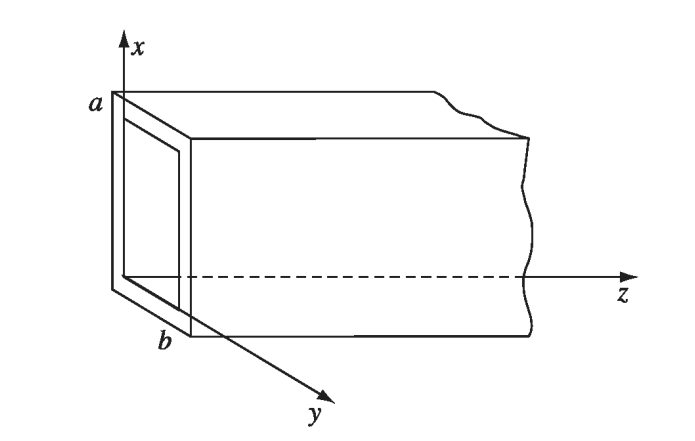
\includegraphics[scale=0.4]{fig/fig-guia-onda-rectangular.png}
\end{center}

\subsubsection{Modos TE:} Analizaremos primero la propagación de modos TE. Entonces debemos encontrar soluciones no-triviales de la ecuación \eqref{EOBzGO} que satisfaga la condición de borde (\ref{CdBGO}b). Usando el método de separación de variables, buscamos soluciones separables de la forma
\begin{equation}
B_z^{0,\rm sep}(x, y) = X(x) Y(y),
\end{equation}
donde las funciones $X(x)$ e $Y(y)$ deben satisfacer
\begin{equation}
\frac{d^2 X}{dx^2} = -k_x^2\,X, \quad \frac{d^2 Y}{dy^2} = -k_y^2\,Y,
\end{equation}
con
\begin{equation}\label{RelDispGOR}
k_x^2 + k_y^2  +k^2 = \frac{\omega^2}{c^2}.
\end{equation} 

La condición de borde en $x=0$ y $x=a$ es $B_x=0$ y la relación \eqref{BxGO} implica entonces que necesariamente $(\partial_xB^0_z)=0$. Esto se traduce en las condiciones $X'(0)=X'(a)=0$. Con esto, las soluciones permitidas son de la forma
\begin{equation}
X(x) \propto \cos(k_x x), \qquad k_x = \frac{m\pi}{a}, \quad m=0,1,2,\dots.
\end{equation}
Similarmente, en los bordes $y=0$ e $y=b$ implican que $(\partial_yB_z)=0$, por lo que las funciones $Y$ deben satisfacer $Y'(0)=Y'(b)=0$. Por lo tanto
\begin{equation}
Y(y) \propto \cos(k_y y), \qquad k_y = \frac{n\pi}{a}, \quad n=0,1,2,\dots.
\end{equation}
Con esto, obtenemos que
\begin{equation}
B^0_z(x, y) = B_0 \cos\left(\frac{m \pi x}{a}\right) \cos\left(\frac{n \pi y}{b}\right).
\end{equation}

Reemplazando en las relaciones \eqref{ExGO}--\eqref{ByGO} obtenemos
\begin{align}
    E^0_x &= \frac{-i\omega}{\omega^2/c^2 - k^2}\left(\frac{n \pi}{b}\right)  B_0\cos\left(\frac{m \pi x}{a}\right) \sin\left(\frac{n \pi y}{b}\right), \label{ExGOTE}\\
    E^0_y &= \frac{i\omega}{\omega^2/c^2 - k^2}\left(\frac{m \pi}{a}\right)  B_0\sin\left(\frac{m \pi x}{a}\right) \cos\left(\frac{n \pi y}{b}\right), \label{EyGOTE}\\
    B^0_x &= -\frac{k}{\omega}E^0_y, \label{BxGOTE}\\
    B^0_y &= \frac{k}{\omega}E^0_x. \label{ByGOTE}
\end{align}
%Podemos ver de aquí que el caso $n=m=0$ no suministra soluciones propagantes, sino 
La relación de dispersión \eqref{RelDispGOR} permite entonces escribir
\begin{equation}\label{kGOR}
k = \sqrt{\frac{\omega^2}{c^2} - \left(\frac{m \pi}{a}\right)^2 - \left(\frac{n \pi}{b}\right)^2}.
\end{equation}
Cada modo TE posible es entonces caracterizado por los valores de $m$ y $n$, y son denotamos como modos TE$_{mn}$. A partir de \eqref{kGOR} vemos que existirá una frecuencia mínima (``cutoff frequency'') $\omega_{mn}$ para cada modo: existirán modos TE propagantes sólo si $\omega>\omega_{mn}$, con
\begin{equation}
\omega_{mn} = c \sqrt{\left(\frac{m \pi}{a}\right)^2 + \left(\frac{n \pi}{b}\right)^2}.
\end{equation}
Si $\omega<\omega_{mn}$ entonces $k$ sería imaginario y no tendríamos una onda propagante, sino un modo que se atenuará exponencialmente.

La solución correspondiente a $m=n=0$ no es un modo propagante, puesto que en este caso $B_z=B_0=\text{cte.}$, $B_x=B_y=0$ y $\vec{E}=\vec{0}$, por lo que en este caso sólo tendremos un campo magnético constate y homogéneo a lo largo de la guía.

 El modo con menor frecuencia de cutoff es el modo TE$_{10}$
\begin{equation}
\omega_{10} = \frac{c \pi}{a},
\end{equation}
que corresponde a una longitud de onda $\lambda_{10}=2\pi c/\omega_{10}=2a$.
Si expresamos \eqref{kGOR} como
\begin{equation}
k = \sqrt{\omega^2 - \omega_{mn}^2},
\end{equation}
entonces podemos escribir la velocidades de fase y grupo de las ondas propagadas como
\begin{equation}
v_{\rm f} = \frac{\omega}{k} = \frac{c}{\sqrt{1 - \left(\frac{\omega_{mn}}{\omega}\right)^2}} > c,
\end{equation}
\begin{equation}
v_{\rm g} = \frac{dk}{d\omega} = c \sqrt{1 - \left(\frac{\omega_{mn}}{\omega}\right)^2} < c.
\end{equation}


El modo TE fundamental, TE$_{10}$
\begin{equation}
E_x=E_z=0, \qquad E_y \propto \sin\left(\frac{\pi x}{a}\right) 
\end{equation}

Podemos reescribir $E_y$ como
\begin{equation}
E_y\propto e^{i(kz+\pi x/a-\omega t)}-e^{i(kz-\pi x/a-\omega t)}.
\end{equation}
Vemos de aquí que este modo puede considerarse como una superposición de dos ondas planas propagándose en diagonal dentro de la guía, con vectores de onda de la forma $\vec{k}_\pm = k\hat{z}\pm(\pi /a)\hat{x}$. El ángulo $\theta$ entre la normal 
\begin{equation}
\cos\theta=\pm\frac{\omega_{nm}}{\omega}
\end{equation}


\subsubsection{Modos TM:}  Si $B_z=0$ entonces buscamos soluciones no triviales para $E_z(x,y)$ que deben satisfacer las condiciones de borde $\vec{E}_z\times\hat{x}=\vec{0}$ en $x=0,a$ y $\vec{E}_z\times\hat{y}=\vec{0}$ en $y=0,b$. Las soluciones separables son entonces de la forma
\begin{equation}
E_z(x, y) = E_0 \sin\left(\frac{m \pi x}{a}\right) \sin\left(\frac{n \pi y}{b}\right)e^{i(kz-\omega t)}, \qquad n,m=1,2,3,\dots.
\end{equation}
La menor frecuencia permitida para los modos TM corresponde al caso en que $n=m=1$, es decir
\begin{equation}
\omega^{\rm TM}_{11}=c\sqrt{\frac{\pi^2}{a^2}+\frac{\pi^2}{b^2}}.
\end{equation}

\subsubsection{Modos TEM:} 

Vemos de \eqref{ExGO}--\eqref{ByGO} que si $E_z=0$ y $B_z=0$ todo el campo se anula, de modo que no existen modos TEM no-triviales en una guía de onda rectangular.

Es posible demostrar que en una guía de ondas completamente hueca, pero de sección transversal arbitratria, no pueden existir modos TEM. En efecto, si $E_z=0$ y $B_z= 0$ entonces la ecuación de Gauss implica que $\partial_xE_x+\partial_yE_y=0$ y la componente $z$ de la ecuación de Faraday implica $\partial_xE_y-\partial_yE_x=0$. Entonces podemos escribir $E_x=-\partial_x\phi$, $E_y=-\partial_y\phi$ con $\nabla^2\phi=0$. Sin embargo, las condiciones de borde (\ref{CdBGO}a) implican que $\phi$ debe ser constante en el borde, y entonces la única solución para $\phi$ es una constante, que implica $E_x=E_y=0$.

\subsection{Guía de onda circular}

Modos TE:
\begin{equation}
B_z^{0,mn}(\rho,\varphi)=B_0J_m(\frac{\beta_{mn}\rho}{R})e^{\pm im\varphi}.
\end{equation}

Modos TM:	
\begin{equation}
E_z^{0,mn}(\rho,\varphi)=E_0J_m(\frac{\alpha_{mn}\rho}{R})e^{\pm im\varphi}.
\end{equation}
Aquí $\alpha_{mn}$ y $\beta_{mn}$ denotan en $n$-ésimo cero de $J_m(x)$ y $J'_m(x)$, respectivamente.

El modo TE$_{11}$ es el que posee la menor frecuencia de corte,
\begin{equation}
\omega_{11}=1.8412\frac{c}{R}.
\end{equation}


\section{Potenciales y transformaciones de gauge}

Las ecuaciones de Maxwell conforman un conjunto de 8 ecuaciones diferenciales
parciales para las 6 componentes del campo electromagnético. A menudo es
\textit{conveniente} reducir el número de variables. Esto puede ser conseguido
expresando los campos en términos de \textbf{potenciales electromagnéticos},
de modo que \textit{las ecuaciones homogéneas de Maxwell sean satisfechas
automáticamente} y el número de campos a determinar se reduce a 4. Estos
potenciales se reducen en los casos estacionarios al conocido potencial
electrostático y al potencial vectorial magnético.

En el caso dinámico general, de (\ref{max2}) podemos concluir que $\vec{B}$
puede ser derivado de un \textbf{potencial vectorial}:
\begin{eqnarray}\label{defA2}
\boxed{\vec{B}=\vec{\nabla}\times \vec{A}.}
\end{eqnarray}
Usando esto en (\ref{max4}), obtenemos:
\begin{equation}
\vec{\nabla}\times \vec{E} = -  \frac{\partial\ }{\partial
t}(\vec{\nabla}\times\vec{A}) = -\vec{\nabla}\times
\frac{\partial\vec{A}}{\partial t},
\end{equation}
es decir,
\begin{eqnarray}
\vec{\nabla}\times \left[ \vec{E} + \frac{\partial \vec{A}}{\partial t} \right]
= \vec{0}.
\end{eqnarray}
De aquí vemos que el campo vectorial dado por la suma $\vec{E} + {\partial
\vec{A}}/{\partial t}$ puede ser escrito como gradiente de un campo escalar, esto es:
\begin{equation}
\vec{E} + \frac{\partial \vec{A}}{\partial t}= - \vec{\nabla}\phi ,
\end{equation}
de donde
\begin{equation}\label{defphi2}
\boxed{\vec{E} =   - \vec{\nabla}\phi - \frac{\partial \vec{A}}{\partial t}.}
\end{equation}
Las ecuaciones (\ref{defA2}) y (\ref{defphi2}) muestran que el campo
electromagnético puede ser escrito en términos de un potencial vectorial
$\vec{A}$ y de un potencial escalar $\phi$. Sin embargo, estas funciones
\textit{no son únicas} para $\vec{E}$ y $\vec{B}$ dados. Es fácil verificar
que el campo electromagnético (y consecuentemente todas las predicciones de la
teoría electromagética) permanece invariante (es decir, con igual valor) bajo las
siguientes transformaciones de los potenciales,
\begin{equation}\marginnote{Transformaciones de gauge}\label{tgg}
\boxed{{\vec{A}}' = \vec{A} - \vec{\nabla}{\chi}, \qquad \phi' =\phi +
\frac{\partial \chi}{\partial t},}
\end{equation}
conocidas como \textbf{transformaciones de gauge} y donde $\chi=\chi(\vec{x},t)$
es una función escalar \textit{arbitraria} del espaciotiempo\footnote{La invariancia
de la teoría electromagnética bajo transformaciones de gauge
desempeña un rol muy importante. La generalización de esta propiedad de
invariancia a \textbf{grupos de simetría interna} permitió formular
teorías consistentes para las \textbf{interacciones débiles} unificadas con la electromagnética (\textbf{electrodébil}) y para la \textbf{interacción fuerte}
(\textit{cromodinámica cuántica}). La \textbf{interacción gravitacional} también puede ser descrita, con algunas peculiaridades, como una \textit{teoría de gauge}.}.

\subsubsection{Ecuaciones de Maxwell inhomogéneas en términos de los
potenciales}
Consideremos el caso de un medio lineal, isótropo y homogéneo. Usando (\ref{defA2}) y (\ref{defphi2}) en las ecuaciones inhomogéneas (\ref{max1}) y (\ref{max3}) encontramos:
\begin{equation}\label{emiap1}
 \nabla^2\phi+\frac{\partial\ }{\partial t}\left(\vec{\nabla}\cdot\vec{A}\right)=-\frac{\rho}{\varepsilon},
\end{equation}
\begin{equation}\label{emiap2}
 \nabla^2\vec{A}-\frac{1}{c^2}\frac{\partial^2\vec{A}}{\partial t^2}-\vec{\nabla}\left(\vec{\nabla}\cdot\vec{A}+\frac{1}{c^2}\frac{\partial\phi }{\partial t}\right)=-\mu\,\vec{J}.
\end{equation}
De esta forma, hemos reducido las ecuaciones de Maxwell a un conjunto de 4 ecuaciones diferenciales parciales para los 4 potenciales. Sin embargo, estas ecuaciones no determinan completamente los potenciales, puesto que las transformaciones de gauge \eqref{tgg} \textit{dejan invariantes} \eqref{emiap1} y \eqref{emiap2}. Esto es natural ya que estas ecuaciones dependen en realidad de los campos eléctrico y magnético, y como vimos las transformaciones de gauge no cambian los valores de estos campos. Además, las ecuaciones \eqref{emiap1} y \eqref{emiap2} están \textit{acopladas}, en el sentido que cada una de estas ecuaciones involucra ambos potenciales electromagnéticos.

Es posible explotar la ``\textbf{libertad de gauge}'' de la electrodinámica (es decir, el hecho que los potenciales no son únicos) para \textit{simplificar algunos cálculos}. Una forma de hacer esto es trabajar con potenciales que satisfagan alguna condición extra o \textbf{gauge}. De hecho, el imponer condiciones extras a los potenciales no sólo es conveniente, sino también \textit{necesario}, ya que las ecuaciones \eqref{emiap1} y \eqref{emiap2} no determinan en forma única los campos $\phi$ y $\vec{A}$. Es posible imponer infinitos gauges diferentes para los potenciales (siempre que sean consistentes con las ecuaciones de Maxwell), pero existen algunos de especial utilidad y popularidad.

\subsubsection{Gauge de Coulomb}
Si el potencial vectorial satisface
\begin{equation}\marginnote{Gauge de Coulomb}\label{gaugeC}
\boxed{ \vec{\nabla}\cdot\vec{A}\stackrel{!}{=}0,}
\end{equation}
se dice que se satisface el \textbf{gauge de Coulomb}, \textbf{gauge de radiación} o \textbf{gauge transversal}. En este caso (\ref{emiap1}) y (\ref{emiap2}) se reducen a
\begin{equation}\label{emiap1GC}
 \nabla^2\phi=-\frac{\rho}{\varepsilon},
\end{equation}
\begin{equation}\label{emiap2GC}
 \nabla^2\vec{A}-\frac{1}{c^2}\frac{\partial^2\vec{A}}{\partial t^2}=-\mu\,\vec{J}+\frac{1}{c^2}\vec{\nabla}\left(\frac{\partial\phi }{\partial t}\right).
\end{equation}

Para probar que \textit{siempre es posible imponer la condición de gauge de Coulomb}, podemos considerar el caso en que inicialmente se trabaje con potenciales $\phi_0$ y $\vec{A}_0$ que no satisfacen la condición (\ref{gaugeC}), es decir, $\vec\nabla\cdot\vec{A}_0\neq 0$, y luego demostrar que es posible realizar una transformación de gauge (\ref{tgg}) con una función $\chi$ tal que los nuevos potenciales sí satisfagan (\ref{gaugeC}). Usando (\ref{tgg}b) requerimos entonces que el nuevo potencial vectorial satisfaga
\begin{equation}
\vec\nabla\cdot\vec{A}=\vec\nabla\cdot(\vec{A}_0-\vec\nabla\chi)\stackrel{!}{=}0.
\end{equation}
Esto implica, como condición necesaria y suficiente, que la función $\chi$ debe satisfacer 
\begin{equation}\label{ePchi}
\nabla^2\chi=\vec\nabla\cdot\vec{A}_0,
\end{equation}
es decir, la ecuación de Poisson con una ``fuente'' conocida ($\vec\nabla\cdot\vec{A}_0$, dados los potenciales originales). Ya que han sido demostrados \textbf{teoremas de existencia} para esta ecuación, es decir, que ella siempre tiene soluciones, queda demostrado que es \textit{posible} imponer el gauge de Coulomb. Note, sin embargo, que la función $\chi$ que determina los nuevos potenciales que satisfacen el gauge de Coulomb \textit{no es única}, ya que si $\chi_1$ es solución de (\ref{ePchi}) entonces $\chi_2=\chi_1+\tilde\chi$ también es solución, siempre que $\tilde\chi$ sea una solución de la ecuación de Laplace ($\nabla^2\tilde\chi=0$). Existe entonces una ``\textbf{libertad remanente}'' para seguir realizando transformaciones de gauge, generadas por funciones $\tilde\chi$ que satisfacen la ecuación de Laplace, y que permiten imponer algunas condiciones\footnote{Ojo: no \textit{cualquier} condición, sino aquellas que sean compatibles con el resto de las condiciones, y con las ecuaciones de Maxwell.} adicionales a los potenciales, siempre dentro de la ``familia de potenciales'' que satisface el gauge de Coulomb.

Una de las conveniencias de este gauge es que \textit{la ecuación (\ref{emiap1GC}) tiene la misma forma que en el caso electrostático}\footnote{Se dice por esto que es ``\textit{coulombiano}'', de ahí uno de los nombres asociados a este gauge.}. Debido a esto, y usando la ``libertad remanente'' mencionada anteriormente, es posible elegir\footnote{!`Pruebe esta afirmación!.} el potencial escalar de la forma siguiente:
\begin{equation}\label{phiGC}
\boxed{ \phi(\vec{x},t)=\frac{1}{4\pi\varepsilon}\int\frac{\rho(\vec{x}',t)}{\left|\vec{x}-\vec{x}'\right|}dV'.}
\end{equation}
Esta solución para el potencial puede entonces ser reemplazada en el lado derecho de \eqref{emiap2GC}. 
%Sin embargo, un cálculo sencillo muestra que este último término cancela la \textit{componente irrotacional} (``longitudinal'') de la corriente. En efecto, asumiendo que las fuentes son localizadas, podemos usar el resultado descrito en el apéndice \ref{Apcamps} y separar la densidad de corriente en una componente longitudinal,  $\vec{J}_{\rm l}$, (o irrotacional, con $\vec\nabla\times\vec{J}_{\rm l}=0$) y una transversal,  $\vec{J}_{\rm t}$, (o solenoidal, con $\vec\nabla\cdot\vec{J}_{\rm t}=0$):
%\begin{equation}
% \vec{J}=\vec{J}_{\rm l}+\vec{J}_{\rm t},
%\end{equation}
%con
%\begin{equation}
% \vec{J}_{\rm l} =-\frac{1}{4\pi}\vec\nabla\int\frac{(\vec\nabla\cdot\vec{J})(\vec{x}')}{|\vec{x}-\vec{x}'|}dV',
%\end{equation}
%\begin{equation}
% \vec{J}_{\rm t} =\frac{1}{4\pi}\vec\nabla\times\int\frac{(\vec\nabla\times\vec{J})(\vec{x}')}{|\vec{x}-\vec{x}'|}dV'.
%\end{equation}
A partir de (\ref{phiGC}), y usando la ecuación de continuidad, podemos escribir el segundo término del lado derecho de \eqref{emiap2GC} sólo en términos de la densidad de corriente, ya que
\begin{eqnarray}
\vec{\nabla}\left(\frac{\partial\phi }{\partial t}\right)&=&  \vec{\nabla}\frac{\partial\ }{\partial t}\left(\frac{1}{4\pi\varepsilon}\int\frac{\rho(\vec{x}',t)}{\left|\vec{x}-\vec{x}'\right|}dV'\right) \\
&=&  \frac{1}{4\pi\varepsilon}\vec{\nabla}\int\frac{\frac{\partial\rho }{\partial t}(\vec{x}',t)}{\left|\vec{x}-\vec{x}'\right|}dV' \\
&=& - \frac{1}{4\pi\varepsilon} \vec{\nabla}\int\frac{(\vec{\nabla}'\cdot\vec{J}')}{\left|\vec{x}-\vec{x}'\right|}dV' .%\\
%&=& \frac{1}{\varepsilon}\vec{J}_{\rm l}.
\end{eqnarray}
Con esto, la ecuación (\ref{emiap2GC}) se reduce a
\begin{equation}\label{emiap3GC}
\boxed{\nabla^2\vec{A}-\frac{1}{c^2}\frac{\partial^2\vec{A}}{\partial t^2}=-\mu\,\vec{J}_{\rm T},}
\end{equation}
donde hemos introducido la \textbf{componente transversal de la densidad de corriente}
\begin{align}
\vec{J}_{\rm T} &:= \vec{J}-\frac{1}{c^2\mu}\vec{\nabla}\left(\frac{\partial\phi }{\partial t}\right) \\
&= \vec{J}+\frac{1}{4\pi} \vec{\nabla}\int\frac{(\vec{\nabla}'\cdot\vec{J}')}{\left|\vec{x}-\vec{x}'\right|}dV'.
\end{align}
Se dice que este campo es \textit{transversal} porque satisface
\begin{equation}
\vec\nabla\cdot\vec{J}_{\rm T}\equiv 0.
\end{equation}

En resumen, \textit{en el gauge de Coulomb el potencial vectorial satisface la  \textit{ecuación de onda inhomogénea}, con un término fuente determinado sólo por la componente transversal de la densidad de corriente}. Además, en este gauge  sólo el potencial vectorial contribuye a los \textbf{campos radiativos}\footnote{Como veremos en el capítulo \ref{caprad}, se dice que un campo electromagnético es radiativo si su contribución a la energía radiada muy lejos de las fuentes (``en el infinito'') es no nula.}. En cambio, el potencial escalar \eqref{phiGC} es no-radiativo como consecuencia de que su valor decae al menos tan rápido como $1/r$ a grandes distancias de la fuente.

El gauge de Coulomb es a menudo usado en regiones donde no hay fuentes presentes. En este caso es posible elegir $\phi=0$, ver \eqref{phiGC}, de modo que toda la información del campo electromagnético está contenida en el potencial vectorial $\vec{A}$.


\subsubsection{Gauge de Lorenz}
Otro gauge común es el \textbf{gauge de Lorenz}\footnote{Nombrado en recuerdo de Ludvig Valentin Lorenz (1829-1891): Matemático y Físico Danés. Ver \url{http://es.wikipedia.org/wiki/Ludvig_Lorenz}, quien consideró esta elección en 1867.}, que usualmente es escrito como
\begin{equation}\marginnote{Gauge de Lorenz}\label{gLorenz}
\boxed{\frac{1}{c^2}\frac{\partial\phi}{\partial t}+\vec{\nabla}\cdot\vec{A}\stackrel{!}{=}0,}
\end{equation}
y que \textit{permite desacoplar las ecuaciones} (\ref{emiap1}) y (\ref{emiap2}).
En efecto, si (\ref{gLorenz}) es satisfecha entonces (\ref{emiap1}) y (\ref{emiap2}) se reducen a
\begin{equation}\label{emiap1gL}
 \nabla^2\phi-\frac{1}{c^2}\frac{\partial^2\phi}{\partial t^2}=-\frac{\rho}{\varepsilon},
\end{equation}
\begin{equation}\label{emiap2gL}
 \nabla^2\vec{A}-\frac{1}{c^2}\frac{\partial^2\vec{A}}{\partial t^2}=-\mu\,\vec{J},
\end{equation}
o, introduciendo el \textbf{operador de onda} (u operador de  d'\,Alembert\footnote{Jean Le Rond d'\,Alembert (1717-1783): matemático, filósofo y enciclopedista francés. Ver \url{http://es.wikipedia.org/wiki/Jean_le_Rond_d\%27Alembert}.}), 
$\Box:= c^{-2}{\partial^2}/{\partial t^2}-\nabla^2$,
\begin{equation}\label{emiap1gL2}
 \Box\phi=\frac{\rho}{\varepsilon},
\end{equation}
\begin{equation}\label{emiap2gL2}
 \Box\vec{A}=\mu\,\vec{J}.
\end{equation}

Análogamente al caso del gauge de Coulomb, puede probarse que \textit{el gauge de Lorenz siempre puede ser impuesto}, considerando que inicialmente se usen potenciales ($\phi_0$ y $\vec{A}_0$) que no lo satisfacen, y mostrando que puede encontrarse una función $\chi$ que genere la transformación de gauge apropiada para que los nuevos potenciales sí la satisfagan. En este caso, la condición sobre la función $\chi$ requerida es que
\begin{eqnarray}
0&\stackrel{!}{=}&\frac{1}{c^2}\frac{\partial\phi}{\partial t}+\vec{\nabla}\cdot\vec{A} \\
&=&\frac{1}{c^2}\frac{\partial\ }{\partial t}\left(\phi_0+\frac{\partial\chi}{\partial t}\right)+\vec{\nabla}\cdot\left(\vec{A}_0-\vec\nabla\chi\right) \\
&=&\left(\frac{1}{c^2}\frac{\partial\phi_0}{\partial t} +\vec{\nabla}\cdot\vec{A}_0\right) +\frac{1}{c^2}\frac{\partial^2\chi }{\partial t^2}-\nabla^2\chi,
\end{eqnarray}
es decir, que satisfaga la ecuación de onda inhomogénea:
\begin{equation}
\Box\chi=-\left(\frac{1}{c^2}\frac{\partial\phi_0}{\partial t} +\vec{\nabla}\cdot\vec{A}_0\right).
\end{equation}
La existencia de soluciones de esta ecuación está garantizada. Análogamente al caso del gauge de Coulomb, la función buscada no es única, sino que existe una libertad remanente para realizar transformaciones de gauge ``dentro del gauge de Lorenz'', generadas por funciones $\tilde\chi$ que satisfagan la ecuación de onda, $\Box\tilde\chi=0$. 

El gauge de Lorenz es usado comúnmente en el contexto de la teoría de Especial de la Relatividad, ya que en el vacío (cuando $\varepsilon=\varepsilon_0$ y $\mu=\mu_0$ y por lo tanto $c=c_0$) la condición (\ref{gLorenz}) así como (\ref{emiap1gL2}) y (\ref{emiap2gL2}), \textit{mantienen su forma inalterada en cualquier sistema de referencia inercial} (son \textit{covariantes} bajo transformaciones de Lorentz). Esto tiene como consecuencia que toda expresión que involucre a los potenciales electromagéticos (que satisfagan el gauge de Lorenz) tendrá la \textit{misma forma en todo Sistema de Referencia Inercial}. Esto no ocurre, por ejemplo, si se usan potenciales que satisfagan el gauge de Coulomb.
